\documentclass[11pt, oneside]{article} 
\usepackage{geometry}
\geometry{letterpaper} 
\usepackage{graphicx}
	
\usepackage{amssymb}
\usepackage{amsmath}
\usepackage{parskip}
\usepackage{color}
\usepackage{hyperref}

\graphicspath{{/Users/telliott/Dropbox/Github-Math/geoproof/figures/}{/Users/telliott/Dropbox/Github-Math/figures/}}
% \begin{center} \includegraphics [scale=0.4] {gauss3.png} \end{center}

\title{Broken Chord}
\date{}

\begin{document}
\maketitle
\Large

%[my-super-duper-separator]

We look at a few problems involving circles, culminating in the broken chord theorem of Archimedes.

\subsection*{a tangent problem}
Two circles of different sizes are shown below with a base line tangent to both, namely $UPRS$.

$TR$ is drawn tangent to both circles, meeting them at point $T$, on the line joining their centers $O$ and $Q$.  Show that $\angle PTS$ is a right angle.
\begin{center} 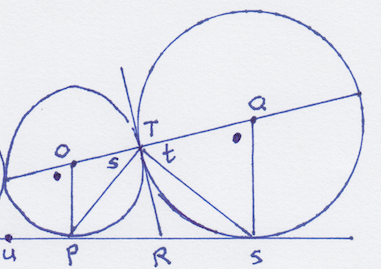
\includegraphics [scale=0.5] {M1.png} \end{center}

\emph{Solution}.

Note first that the blue dotted angles, one at $O$, supplementary to $\angle POT$, and the other one at $Q$, namely $\angle TQS$, are equal, by similar triangles. 

$\triangle OPT$ is isosceles (two radii of the circle on center $O$), so $2s$ is equal to the blue dotted angle by the exterior angle theorem.  $\triangle TQS$ is also isosceles, for the same reason, so $2t$ is supplementary to the blue dotted angle by the angle sum theorem.  \[ 2s + 2t = 180 \]
We conclude that $s + t$ is a right angle, so $\angle PTS$ is also, by supplementary angles.

There are other approaches, e.g. the quadrilaterals $POTR$ and $RTQS$ are similar with two right angles and one copy each of the blue dotted angle and its supplement.

$\square$

\subsection*{rectangle extensions}

In the figure below, $ABCD$ is a rectangle inscribed in a circle.  $PQ$ is drawn parallel to $BC$, forming rectangle $EBCF$. 

$OT \perp BC$.  Show that $PE = FQ$.
\begin{center} 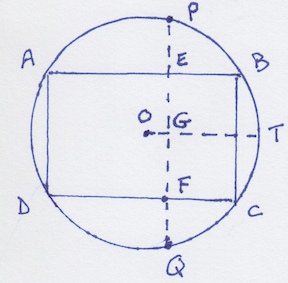
\includegraphics [scale=0.6] {M2.png} \end{center}

\emph{Solution}.

$\triangle OBC$ is isosceles.  Since $OT \perp BC$ and goes through the vertex $O$ of $\triangle OBC$, the base of the isosceles triangle $BC$ is bisected by $OT$.  Refer to the standard proof of the isosceles triangle theorem.

Then, $PQ \parallel BC$.  But $\triangle OPQ$ is also isosceles, so $PQ$ is also bisected by $OT$, which means that $PG = GQ$.

Since $EBCF$ is a rectangle and $OT$ is the perpendicular bisector of one side $BC$, it is also the perpendicular bisector of the other side, $EF$.  So $EG = GF$.

\[ PG = GQ \]
\[ BT = TC = EG = GF \]
so
\[ PG - EG = GQ - GF \]
The left-hand side is $PE$ and the right-hand side is $FQ$.  Hence
\[ PE = FQ \]

$\square$

\subsection*{extraordinary property of the circle}

Two perpendicular chords are drawn $AB$ and $EF$.  They may cross anywhere in the circle.  The pieces are $a$, $b$, $c$ and $d$.  The radius of the circle is $R$.

Show that $a^2 + b^2 + c^2 + d^2 = 4R^2$.
\begin{center} 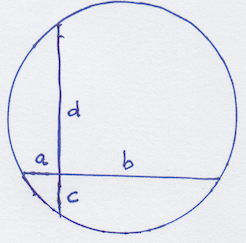
\includegraphics [scale=0.6] {M3a.png} \end{center}
We draw the rectangle $ABCD$ and its diagonals $AC$ and $BD$ (below).

These are also diagonals of the circle, by the converse of Thales theorem.  Given that $\angle DAB$ is a right angle, it follows that $BD$ is a diagonal.  

Two diagonals of a circle cross at a single point, and they both go through the center, so that's where they must cross.  (Alternatively, use congruent triangles).

The length of the rectangle is $a + b$.  The length of $FG$ is $d$.  The parts of $FE$ that lie outside the rectangle are both equal, that is, $c$.  This is the previous result.  As a result, we have that the width of the rectangle is $d - c$.

\begin{center} 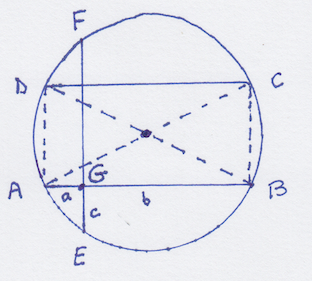
\includegraphics [scale=0.6] {M3b.png} \end{center}
Apply the Pythagorean theorem
\[ (a + b)^2 + (d - c)^2 = (2R)^2 \]
\[ a^2 + 2ab + b^2 + c^2 - 2cd + d^2 = 4R^2 \]

As the arms of chords that cross in a circle, we showed previously that $ab = cd$.  With the cancelation, we have
\[ a^2 + b^2 + c^2 + d^2 = 4R^2 \]

$\square$

\subsection*{the broken chord, I}

The theorem of the ”broken chord” is ascribed to Archimedes, although his original work has been lost. It was analyzed by the Arabic mathematician Al'Biruni in his \emph{Book on the Derivation of Chords in a Circle}.

Pick two points on a circle, $A$ and $C$ and let $M$ lie midway between them.  If the chords $AM$ and $MC$ were drawn, they would be equal.  Now pick $B$ to one side of $M$ and draw $AB$ and $BC$.

Drop the perpendicular from $M$ to $BC$ at $F$.

I claim that $AB + BF = FC$.
\begin{center} 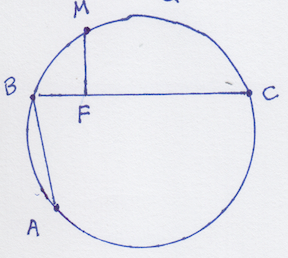
\includegraphics [scale=0.6] {M4a.png} \end{center}

\emph{Proof}.

The clever idea is to place point $E$ such that $AB = EC$ (below).  

Now, if we can show that $\triangle BME$ is isosceles, then $MF$ bisects the base and we are done.

By the property of the midpoint, we know that $AM = MC$.  Having drawn those chords, we notice that $\angle A$ and $\angle C$ subtend the same arc of the circle, so they are equal.  The other flanking side is $AB$ which is equal to $EC$ by our construction.
\begin{center} 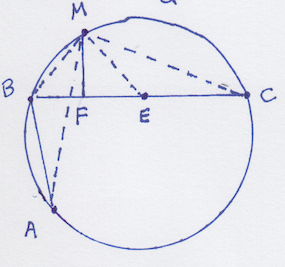
\includegraphics [scale=0.6] {M4b.png} \end{center}
Thus, we have two congruent triangles by SAS.  $\triangle ABM \cong \triangle ECM$.
  
Since they are corresponding parts of congruent triangles, $BM = ME$.  

That means $\triangle BME$ is isosceles.  Since $MF$ is the perpendicular to base $BE$, it bisects it, by the properties of isosceles triangles.

We have that $BF = FE$, and $AB = EC$, so their sums are equal as well.  $AB + BF = FE + EC = FC$.

$\square$

\subsection*{the broken chord, II}

There is another neat proof of this theorem.  

\emph{Proof}.

Draw the rectangle $MGEF$.  By the work on parallel chords earlier in this chapter, we know that $BF = EC$.
\begin{center} 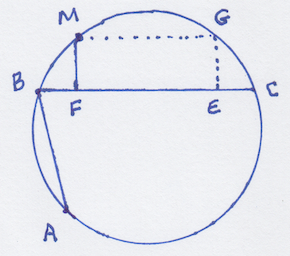
\includegraphics [scale=0.6] {M4c.png} \end{center}

Hence we have two small congruent triangles $\triangle BFM \cong \triangle GEC$ by SAS, and so it follows that $BM = GC$.  

Chords of equal length in a given circle have the same arc and vice-versa.  Furthermore, arc lengths are additive, though chord lengths are not (See below).

Hence the arcs $BM$ and $GC$ are equal as are $AM$ and $MC$, so by subtraction $AB = MG$.  So the chords corresponding to those arcs, $AB$ and $MG$ are also equal.

But $MG$ and $FE$ are opposite sides in a rectangle.  It follows that $AB = FE$.

By addition, $AB + BF = FE + EC$.

$\square$

The first proof duplicated the length $AB$ with $C$ as the endpoint, while this proof duplicates the length $BF$ with $C$ as the endpoint.

\subsection*{arcs and chords}

We said that chords of equal length in a given circle have the same arc and vice-versa.  We haven't stated this relationship explicitly so far.

The measure of an angle $\theta$ is the length of arc $s$ that it subtends \emph{in a unit circle}.  Hence $\theta$ gives us $s$ and $s$ gives us $\theta$, and of course, any peripheral angle subtending the same arc as a central angle is just one-half that angle.

There is a difference between arcs and chords, however.  Arcs add (as do angles), but chords do not.  A simple reason is the triangle inequality.

Anticipating the chapter on basic trigonometry, we consider the chord corresponding to a central angle of $2 \theta$ in a unit circle, and introduce the sine of that angle $\theta$ as one-half of the chord.  This also corresponds to one-half the chord subtended by a peripheral angle of $\theta$.
\begin{center} 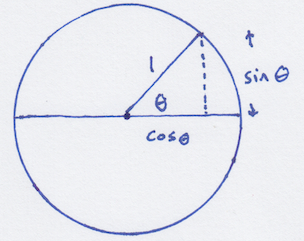
\includegraphics [scale=0.7] {L1b.png} \end{center}

Both sine and its inverse are functions.  The sine returns a unique value in the range $[0,1]$ for any input in the range $0-90$ degrees  (For radian measure, see the chapter on basic trigonometry).  Both functions are increasing everywhere on their intervals.  This means that any angle corresponds to a unique chord, and any chord corresponds to a unique angle.

The arc determines the angle determines the chord, and vice-versa.

It will turn out that to add chords, we must adjust the lengths.  We will show later that
\[ \sin \theta + \phi = \sin \theta \cos \phi + \sin \phi \cos \theta \]
\begin{center} 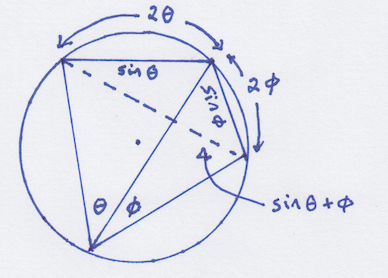
\includegraphics [scale=0.6] {M6.png} \end{center}
Each of the smaller chords is shrunk by an amount equal to the cosine of the same angle.  This shrinkage is larger (as a percentage) as the measure of the angle is greater, since the cosine gets closer to $0$.

The result that we need for this chapter is that if two arcs of a circle are equal, then so are the chords of those arcs, and vice-versa.

\end{document}